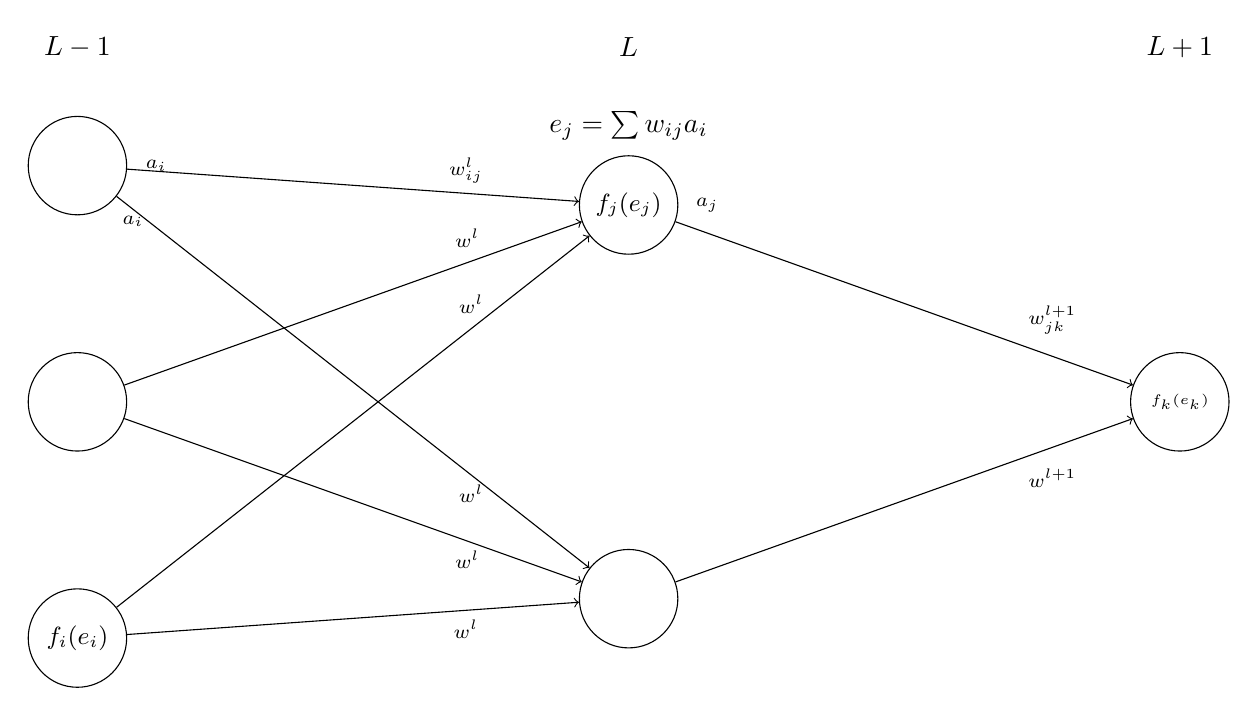
\begin{tikzpicture}

	\tikzstyle{nodo}=[circle, draw, minimum size=1.25cm]
	\tikzstyle{upw}=[dashed, red, ->, line width = 1pt]

	\coordinate (l_0) at (0, 4.5);
	\coordinate (l_1) at (7, 4.5);
	\coordinate (l_2) at (14, 4.5);

	\coordinate (f_1_1) at (0, 3); % CAPA ENTRADA
	\coordinate (f_1_2) at (0, 0); % CAPA ENTRADA
	\coordinate (f_1_3) at (0, -3); % CAPA ENTRADA
	\coordinate (f_2_1) at (7, 2.5); % CAPA OCULTA 1
	\coordinate (f_2_2) at (7, -2.5); % CAPA OCULTA 1
	\coordinate (f_3_1) at (14, 0); % CAPA SALIDA

	\node[] (l_0) at (l_0) {$L - 1$};
	\node[] (l_1) at (l_1) {$L$};
	\node[] (l_2) at (l_2) {$L + 1$};

	\node[nodo] (f_1_1) at (f_1_1) {}; % CAPA ENTRADA
	\node[nodo] (f_1_2) at (f_1_2) {}; % CAPA ENTRADA
	\node[nodo] (f_1_3) at (f_1_3) {\small $f_i(e_i)$}; % CAPA ENTRADA
	\node[nodo] (f_2_1) at (f_2_1) {\small $f_j(e_j)$}; % CAPA OCULTA 1
	\node[nodo] (f_2_2) at (f_2_2) {}; % CAPA OCULTA 1
	\node[nodo] (f_3_1) at (f_3_1) {\tiny $f_k(e_k)$}; % CAPA SALIDA


	\draw[->, font=\scriptsize] (f_1_1) node[right of=f_1_1] {$a_{i}$} -- node[pos=0.75, above] (w_1_1) {$w^{l}_{ij}$} (f_2_1);
	\draw[->, font=\scriptsize] (f_1_2) node[below right of=f_1_1] {$a_{i}$} -- node[pos=0.75, above] (w_1_2) {$w^{l}_{}$} (f_2_1);
	\draw[->, font=\scriptsize] (f_1_3) -- node[pos=0.75, above] (w_1_3) {\scriptsize$w^{l}_{}$} (f_2_1);
	\draw[->, font=\scriptsize] (f_1_1) -- node[pos=0.75, below] (w_2_1) {$w^{l}_{}$} (f_2_2);
	\draw[->, font=\scriptsize] (f_1_2) -- node[pos=0.75, below] (w_2_2) {$w^{l}_{}$} (f_2_2);
	\draw[->, font=\scriptsize] (f_1_3) -- node[pos=0.75, below] (w_2_3) {$w^{l}_{}$} (f_2_2);

	\node[above of=f_2_1] {$e_{j} = \sum w_{ij}a_i$};

	\draw[->, font=\scriptsize] (f_2_1) node[right of=f_2_1] {$a_{j}$} -- node[pos=0.75, above right] (w_j_k) {$w^{l+1}_{jk}$} (f_3_1);
	\draw[->, font=\scriptsize] (f_2_2) -- node[pos=0.75, below right] {$w^{l+1}$} (f_3_1);


	%\draw[upw] (f_3_1) to[bend left=20] (w_1_1);
	%\draw[upw] (f_3_1) to[bend left=20] (w_1_2);
	%\draw[upw] (f_3_1) to[bend left=20] node[pos=0.7, right] {$w^{l}_{ij} - \alpha\frac{\partial e}{\partial w}$} (w_1_3);


	%\draw[upw] (f_4_1) to[bend right=20] node[pos=0.8, right] {$w^{l+1}_{jk} - \alpha\frac{\partial e}{\partial w^{l+1}_{jk}}$} (w_j_k);

	%\node[above right of=w_j_k, node distance=3cm] {$\frac{\partial e}{\partial w^{l+1}_{jk}}=-(s_i - y_i)\frac{\partial y_i}{\partial w^{l+1}_{jk}}$};
\end{tikzpicture}
